\chapter{Multi-domain residual adapters}
\label{chap:res}
\section{Introduction}
In \emph{supervised multi-domain adaptation} discussed in Section \ref{sec:case1}, the fine-tuning method \citep{Luong15stanford,Freitag16fast} usually achieve the best performance in single domain adaptation. However, fine-tuned models are usually brittle to out-of-domain examples. Therefore, it is only suitable for the "one domain one model" strategy, which requires much effort for maintenance and training. Several recent studies \citep{Vilar18learning,Wuebker18compact,Michel18extreme,Bapna19simple} have proposed more lightweight schemes to perform domain adaptation while also preserving the value of pre-trained models. Our main inspiration is the latter work, whose proposal relies on small \emph{adapter components} \citep{Bapna19simple} that are plugged in each hidden layer. These adapters are trained only with the in-domain data, keeping the pre-trained model frozen. \citet{Bapna19simple} used the adapters for MT domain adaptation and multilingual MT. Because these additional adapters are very small compared to the size of the baseline model, their use significantly reduces the cost of training and maintaining fine-tuned models while delivering a performance that remains close to that of full fine-tuning.

In this chapter, we conduct a thorough analysis of the adapter model in the context of a multi-domain machine translation task. We notably explore ways to adjust and/or regularize adapter modules to handle situations where the adaptation data is minimal. We also propose and contrast two new variants of the residual architecture: in the first one (\emph{highway residual adapters}), adaptation still affects each layer of the architecture, but its effect is delayed till the last layer, thus making the architecture more modular and adaptive; our second variant (\emph{gated residual adapters}) exploits this modularity and enables us to explore ways to improve performance in the face of train-test data mismatch. We experiment with two language pairs and report results that illustrate the flexibility and effectiveness of these architectures. Our main conclusions are that residual adapters provide a fast and relatively low-cost method (compared to fine-tuned systems) for supervised multi-domain adaptation; our two variants prove as effective as the original adapter model and open perspectives to make adapted models more robust to label domain errors.

\textit{This chapter draws from the following publications: \citet{Pham20Study}}.
\section{Residual adapters \label{sec:res-chap6}}
In this section, we describe the basic version of the residual adapter architectures \citep{houlsby19parameter, Bapna19simple}, as well as two novel variants of this model.

\subsection{Basic architecture \label{ssec:architecture-chap6}}
\fyDone{More contexts and notations from the transformer}\fyDone{Encoder / decoder layers}

\subsubsection{The computation of adapter layers}
Our reference architecture is the Transformer model of \citet{Vaswani17attention}, which we assume contains a stack of layers both on the encoder and the decoder sides. Each layer contains two subparts, an attention layer, and a dense layer. Details vary from one implementation to another, we simply contend here that each layer $i \in \{1 \dots L\}$ (in the encoder or the decoder) computes a transform of a fixed-length sequence of $d$-dimensional input vectors $h^{i}$ into a sequence of output vectors $h^{i+1}$ as follows ($\mathbf{LN}$ denotes the (sub)layer normalization, $\mathbf{ReLU}$ is the ``rectified linear unit'' operator):\fyDone{Use align env}\fyDone{Add layer normalization, replace notation b by a}
\begin{align*}
  h^{i}_0 &= \mathbf{LN}(h^{i}) \\
  h^{i}_1 &= \mathbf{W}_{db}^{i}h_0^{i} + a^i_{1} \\
  h^{i}_2 &= \mathbf{ReLU}(h_1^{i})
  \\
%\end{align*}
%\begin{align*}
  h^{i}_3 &= \mathbf{W}_{bd}^{i}h_2^{i} + a^i_{2} \\
  \bar{h}^{i} &= h^{i}_3 + h^i.
\end{align*}
Overall, the  $i^{\text{th}}$ adapter is thus parameterized by matrices $\displaystyle{\mathbf{W}_{db}^{i}\in\mathbb{R}^{d\times b}}$,$\displaystyle{\mathbf{W}_{bd}^{i}\in\mathbb{R}^{b\times d}}$, bias vectors $\displaystyle{b^i_{1} \in \mathbb{R}^{b}}$, $\displaystyle{b^i_{2} \in \mathbb{R}^{d}}$, with $b$ the dimension of the adapter \fyDone{($d \gg b$) not true}\fyDone{Check this}. For the sake of brevity, we will simply denote $h^{i}_3 = \operatorname{ADAP}^{(i)}(h^i)$, and $\theta_{\operatorname{ADAP}^{(i)}}$ the corresponding set of parameters.\fyDone{or is it $h_i$ ?}\fyDone{attention aux matrices $W_i$}

The "adapted" hidden vectors $\bar{h}^i_{ 1\leq i \leq L-1}$, where $L$ is the number of layers, will then be the input of the $(i+1)^{\text{th}}$\fyDone{Self attention ?} layer; $\bar{h}^L$ is passed to the decoder if it belongs to the encoder side, or is the input of output layer if it belongs to the decoder side. Note that zeroing out all adapters enables us to recover the basic Transformer, with $\bar{h}^{i} = h^i$ for all $i$.

In the experiments of Section~\ref{sec:exp-chap6}, we use $2\times{}L=12$ residual adapters, one for each of the $L=6$ attention layers of the encoder and similarly for the decoder.\footnote{In the decoder, the stack of self-attention and cross encoder-decoder attention only counts as one attention layer and only corresponds to one residual adapter.}

\subsubsection{Design space and variants}
\label{sssec:design-space-chap6}
This general architecture leaves open many design choices pertaining to the details of the network organization, the training procedure, and the corresponding objective function.

The first question is the number of adapter layers. While in principle, all Transformer layers can be subject to adaptation, it is nonetheless worthwhile to consider simpler adaptation schemes, which would only alter a limited number of layers. Such strategys might be especially relevant when the training data contains very small domains, as in the experiments of Section~\ref{sec:exp-chap6}, and for which a complete adaptation may not be necessary or/and or prone to overfitting. This, in turn, raises the issue of which layer(s) to adapt, a question that can be approached in the light of recent analyses of Transformers models, which conjecture that the higher layers encode global patterns with a more ``semantic'' interpretation, while the lower layers encode local patterns akin to morpho-syntactic information \cite{raganato18analysis}.

Beside the reduction of the numbers of adapters in a model, we can apply smooth regularization methods to mitigate overfitting. Our first proposition is to use weight decay \citep{Krogh91simple}. The method proposes adding a second term, which is the norm $L_2$ of the model's parameters, to cross-entropy loss as follows
\begin{equation*}
  \begin{array}{rcl}
  \bar{L} & = &  E_{x \sim \mathcal{D}_e^d(x), y \sim g^d(x)} [-log(P(y|x,\theta_d))] \\
    & + & \lambda  \sum_{i \in \{1,..,6\} \otimes \{enc, dec\}} \normL{\theta_{\operatorname{ADAP}^{(i)}_{(d)}}}
  \end{array}
\end{equation*}
in which $d$ is the target domain, variables $\theta_{\operatorname{ADAP}^{(i)}_{(d)}}$ belongs to $\theta_d$ and $\theta_d \setminus \{ \theta_{\operatorname{ADAP}^{(i)}_{(d)}} \}_{i \in \{1,..,6\} \otimes \{enc, dec\}}$ are frozen during the training.
We reuse the same notations as in Equation ~\refeq{eq:loss-chap5}.

An alternative scheme is \emph{layer regularization}, which penalizes the output of the adapters, corresponding to the following objective:
\begin{equation*}
  \begin{array}{rcl}
    \bar{L} & = &  E_{x \sim \mathcal{D}_e^d(x), y \sim g^d(x)} \big[-log(P(y|x,\theta_d)) \\
    & + & \lambda \sum_{i \in \{1,..,6\} \otimes \{enc, dec\}} \normL{\operatorname{ADAP}^{(i)}(h_i(x,y))} \big]
  \end{array}
\end{equation*}

Finally, another independent design choice relates to the training strategy for adapters. A first option is to generalize supervised domain adaptation to multi-domain adaptation and to proceed in two steps: (a) train a generic model with all the available data; (b) train each adapter layer with domain-specific data, keeping the generic model parameters unchanged. Another strategy is to adopt the view of \citet{Dredze08online}, where the multi-domain setting is considered as an instance of multi-task learning \cite{Caruana97multitask} with each domain corresponding to a specific task. This suggests training all the parameters from scratch, as we would do in a multi-task mode. The generic parameters will still depend on all the available data, while each adapter will only be trained with the corresponding in-domain data.\fyFuture{Does everyone need a domain? Do we need this discussion - talk about sentence-level adaptation, better classifier pour MDL}

\subsection{Highway Residual Adapters \label{ssec:highway-chap6}}

In the basic architecture described in Section~\ref{ssec:architecture-chap6}, the computation performed by lower-level layers will impact all the subsequent layers. This section introduces a variant of residual adapters, which delays the adaptation of each layer to the last layers (of the encoder and the decoder). We demonstrate our proposal in Figure~\ref{fig:hrl-architecture-chap6}. While the basic architecture performs adaptation in sequence, we propose here to perform it in parallel. In this version, only the last hidden vector of the encoder (decoder) is thus modified according to:
\begin{equation}
  \bar{h}^L = h^L + \displaystyle{\mathop{\sum}_{1 \leq i \leq L} ADAP^i(h^i)} \label{eq:highway-output-chap6}
\end{equation}

One obvious benefit of this variant is that it allows us to reuse the hidden vectors $h^i$ of all hidden layers when computing an adapted output for several domains during the inference. In this situation, the forward step only needs to compute the hidden vectors $h^i$ once for the inner encoder layers before an adapted sequence of vectors is computed at the topmost layer. Therefore, we can fine-tune the model to multiple domains at once without recomputing $h^i$. This variant also opens the way to more parameter sharing across adapters, a perspective that we will not explore further in this work. Instead, we use it to develop a second variation of the adapter model, which is presented in the next section.

\begin{figure}[htbp]
  \centering
  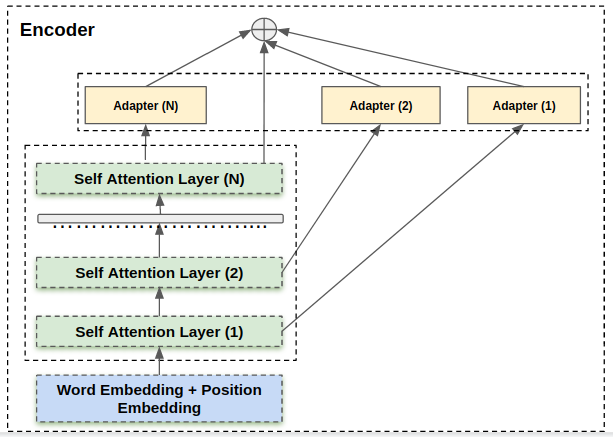
\includegraphics[scale=0.3]{graphics/highway_residual}
  \caption{Highway residual adapter network}
  \label{fig:hrl-architecture-chap6}
\end{figure}

\subsection{Gated Residual Adapters \label{ssec:gate-chap6}}
\mpDone{Formalizing problem, network design, training algorithm}
The basic architecture presented above rests on a rather simplistic view of ``domains'' as made of well-separated and unrelated pieces of texts that are processed independently during adaptation. Likewise, when translating test documents, one needs to choose between either using one specific domain-adapted model or resorting to the generic model. In this context, using wrong domain labels can have a strong (negative) effect on translation performance. 

Therefore, we would like to design a version of residual adapters that is more robust to such domain errors. This variant, called the \emph{gated residual adapter model}, relies on the training of a supplementary component that will help decide whether to activate, on a word per word basis, a given residual layer and to regulate the strength of this activation. To this end, we extend the highway version of residual adapters as follows.
\fyDone{Consistency of notations wrt section 2.1}

Formally, we replace the adapter computation of equation~\eqref{eq:highway-output-chap6} and take the adapted hidden (topmost) layer to be computed as (this is for domain $k$):
\begin{equation}
  \bar{h}^L = h^L + \displaystyle{\mathop{\sum}_{1 \leq i \leq L} \operatorname{ADAP}_k^i(h^i) \odot{} z_k(h^L)}, \label{eq:gated-output-chap6}
\end{equation}
where the scalar $z_k(h^L[t]) \in [0,1]$ measures the relatedness of the $t^{\text{th}}$ word $w_t$ to domain $k$. The more likely $w_t$ is in domain $k$, the larger $z_k(h^L[t])$ should be; conversely, for words\footnote{The term ``word'' is employed here by mere convenience, as systems only manipulate sub-lexical BPE units; furthermore, the values of the hidden representations $h^{i}$ at position $t$ depend upon all the other positions in the sentence.} that are not typical of any domain $k$ (eg.\ function words),  adaptation is minimum and the corresponding adapted encoder output ($\bar{h}^L[t]$) will remain close to the output of the generic model ($h^L[t]$). In our implementation, we incorporate two domain classifiers on top of the encoder and the decoder, that take the last hidden layer of the encoder (resp.\ decoder) as input and use the posterior probability $P(k|h^L[t])$ of domain $k$ as the value for $z_k(h^L[t])$.

Training gated residual adapters thus comprises three steps, instead of two for the baseline version:
\begin{enumerate}
\item learn a generic model with mixed corpora from multiple domains.
\item train a domain classifier on top of the encoder and decoder; during this step, the parameters of the generic model are frozen. This model computes the posterior domain probability $P(k|h^L[t])$ for each word $w_t$, based on the representation computed by the last layer.
\item train the parameters of adapters with in-domain data separately for each domain, while freezing all the other parameters.
\end{enumerate}
\fyFuture{is this classifier important, can we train with the rest of the system? Yes we could, but do we want the encoder to be good at classification?}\fyFuture{Check writing to indicate label smoothing for this has been used.}\fyFuture{Can we train a more complex training model ? should we use more monolingual data? etc} 

\section{Experimental settings \label{sec:exp-chap6}}

\subsection{Data and metrics \label{ssec:corpora-chap6}}
We perform our experiments with two translation pairs involving multiple domains: English-French (En$\rightarrow$Fr) and English-German (En$\rightarrow$De). For the former pair, we use texts\footnote{Most corpora are available from the Opus web site: \url{http://opus.nlpl.eu}} initially from 6~domains, corresponding to the following data sources: the UFAL Medical corpus V1.0 (\domain{med})\footnote{\url{https://ufal.mff.cuni.cz/ufal_medical_corpus}}, the European Central Bank corpus (\domain{bank}) \cite{Tiedemann12parallel}; The JRC-Acquis Communautaire corpus (\domain{law}) \cite{Steinberger06acquis}, documentations for KDE, Ubuntu, GNOME and PHP from Opus collection \cite{Tiedemann09news}, collectively merged in a \domain{it}-domain, Ted Talks (\domain{talk}) \cite{Cettolo12wit}, and the Koran (\domain{rel}). Complementary experiments also use v12 of the News Commentary corpus (\domain{news}). Corpus statistics are in Table~\ref{tab:Corpora-en-fr-chap6}.  

\begin{table*}[htbp]
  \centering
  \begin{tabular}{ |lllllll|} %*{4}{|r|}}
    \hline
    %\multicolumn{4}{|l|}{Vocab size - En: 30,165, Fr: 30,398}\\
    \domain{med} & \domain{law} & \domain{bank} & \domain{it} & \domain{talk} & \domain{rel} & \domain{news} \\
    \hline
    2609 (0.68) & 190 (0.05)  & 501 (0.13) & 270 (0.07) & 160 (0.04) & 130 (0.03) & 260 (0) \\
    \hline
  \end{tabular}
\caption{Corpora statistics for En$\rightarrow$Fr : number of parallel lines ($\times 10^3$) and proportion in the basic domain mixture (which does not include the \domain{news} domain). \domain{med} is the largest domain, containing almost 70\% of the sentences, while \domain{rel} is the smallest, with only 3\% of the data.}
\label{tab:Corpora-en-fr-chap6}
\end{table*}

En$\rightarrow$De is a much larger task, for which we use corpora distributed for the News task of WMT20\footnote{\url{http://www.statmt.org/wmt20/news.html}} including: European Central Bank corpus (\domain{bank}),  European Economic and Social Committee corpus (\domain{eco}), European Medicines Agency corpus (\domain{med})\footnote{\url{https://tilde-model.s3-eu-west-1.amazonaws.com/Tilde_MODEL_Corpus.html}}, Press Release Database of European Commission corpus, News Commentary v15 corpus, Common Crawl corpus (\domain{news}), Europarl v10 (\domain{gov}), Tilde MODEL - czechtourism (\domain{tour})\footnote{\url{https://tilde-model.s3-eu-west-1.amazonaws.com/Tilde_MODEL_Corpus.html}}, Paracrawl and Wikipedia Matrix (\domain{web}). Statistics are in Table~\ref{tab:Corpora-en-de-chap6}.
\begin{table*}[htbp]
  \centering
  \begin{tabular}{ |lllllll|} %*{4}{|r|}}
    \hline
    %\multicolumn{4}{|l|}{Vocab size - En: 30,165, Fr: 30,398}\\
    \domain{bank} & \domain{eco} & \domain{med} & \domain{gov} & \domain{news} & \domain{tour} & \domain{web} \\
    \hline
    4 (0.00022) & 2857 (0.15) & 347 (0.018) & 1828 (0.095) & 3696 (0.19) & 7 (0.00039) & 10473 (0.54) \\
    \hline
  \end{tabular}
\caption{Corpora statistics for En$\rightarrow$De: number of parallel lines ($\times 10^3$) and proportion in the basic domain mixture. \domain{web} is the largest domain, containing about 54\% of the sentences, while \domain{bank} and \domain{tour} are very small.}
\label{tab:Corpora-en-de-chap6}
\end{table*}

We randomly select in each corpus a development and a test set of 1,000 lines each and keep the rest for training.\footnote{Scripts to replicate these experiments are available at url{https://github.com/qmpham/experiments.git}.} Development sets help choose the best model according to the average BLEU score \cite{Papineni02bleu}.\footnote{We use truecasing and the \texttt{multibleu} script.}\fyDone{A word about meta-parameter settings}

\subsection{Baseline architectures \label{ssec:baseline-chap6}}
Using Transformers implemented in OpenNMT-tf\footnote{\url{https://github.com/OpenNMT/OpenNMT-tf}} \cite{Klein17opennmt}, we train the following baselines:
\begin{itemize}
\item a generic model trained on a concatenation of all corpora, denoted \system{Mixed-Nat};
\item a fine-tuned model \citep{Luong15stanford,Freitag16fast}, based on the \system{Mixed-Nat} system, denoted \system{FT-Full}
\end{itemize}
The description of these systems and their implementations can be found in Section ~\ref{ssec:baselines-chap4} and Appendix \ref{appendix:a}.

For all En$\rightarrow$Fr models, we set the embeddings size and the hidden layers size to~512. Transformers use multi-head attention with 8 heads in each of the 6 layers; the inner feedforward layer contains 2,048 cells. Residual adapters additionally use an adaptation block in each layer, composed of a 2-layer perceptron, with an inner ReLU activation function operating on normalized entries of dimension $b=1024$. \citet{Bapna19simple} showed that the performance of adapted models increases with respect to the size of the inner dimension and obtained performance close to the full fine-tuned model with $b=1024$, which is twice as large as the dimension of a Transformer layer. We used the same setting in our experiments.\fyDone{Check: is it $b$?}

Training uses a batch size of~12,288 tokens; optimization uses Adam with parameters $\beta_1=0.9$, $\beta_2= 0.98$ and Noam decay ($warmup\_steps=4,000$), and a dropout rate of $0.1$ for all layers. For the \system{Mixed-Nat} model, we use an initial learning rate of $1.0$ and take the concatenation of the validation sets of 6~domains for development. In the fine-tuning experiments, we continue training using \system{Mixed-Nat} as starting point, using the same learning rate schedule, and continuing the incrementation of the number of steps. In the multi-task training, we use the same learning rate schedule as for \system{Mixed-Nat}: for each iteration, we sample a domain a probability proportional to its size; we then sample a batch of~12,288 tokens that is used to update the shared parameters and the parameters of the corresponding adapter.\fyDone{Describe the block adaptation layer - voir slides}

Models for En$\rightarrow$De are larger and rely on embeddings as well as hidden layers of size~1024; each Transformers layer contains 16~attention heads; the inner feedforward layer contains 4,096 cells. Adapter modules have the same architecture as for the other language pair, except for their size, which is doubled ($b=2,048$).

\iffalse{
\begin{table*}[htbp]
  \centering
  \begin{tabular}{|l|l|} \hline
    Model & params \\ \hline 
    \system{Transformer-En-Fr}  & 65 \\
    \system{Residual Adapter-En-Fr} & 1 \\
    \system{Transformer-En-De}  & 213 \\
    \system{Residual Adapter-En-De} & 4 \\
     \hline
  \end{tabular}
  \caption{Number of parameters ($\times 10^6$)}
  \label{tab:params-chap6}
\end{table*}
}
\fi

\subsection{Multi-domain systems}
In this section, we evaluate several proposals from the literature on multi-domain adaptation and compare them to full fine-tuning on the one hand, and to two variants of the residual adapter architecture on the other hand.
The reference methods included in our experiments are the following:
\begin{itemize}
\item a system using ``domain control'' \citep{Kobus17domain}. In this approach, domain information is introduced either as an additional token for each source sentence (\system{DC-Tag}) or in the form of a supplementary feature for each word (\system{DC-Feat});
\item a system using lexicalized domain representations presented in Chapter~\ref{chap:ldr} (\system{LDR});
\item the three proposals of \citet{Britz17effective}. \system{TTM} is a feature-based approach where the domain tag is introduced as an extra word \textsl{on the target side}. The training uses reference tags and inference is performed with predicted tags, just like for regular target words. \system{DM} is a multi-task learner where a domain classifier is trained on top of the MT encoder, so as to make it aware of domain differences; \system{ADM} is the adversarial version of \system{DM}, pushing the encoder towards learning domain-independent source representations. These methods only use domain labels in training.
\end{itemize}
The description and the implementation of each MDMT system are provided in Appendix ~\ref{appendix:a} and Section ~\ref{ssec:baselines-chap4}.
\begin{table*}[t!]
  \centering
  \begin{tabular}{|p{3.5cm}|*{8}{r|}} \hline
%     &&&&&& \\
    Model / Domain & \multicolumn{1}{c|}{\domain{ med}} & \multicolumn{1}{c|}{\domain{ law}} & \multicolumn{1}{c|}{\domain{bank}} & \multicolumn{1}{c|}{\domain{talk}} & \multicolumn{1}{c|}{\domain{ it }} & \multicolumn{1}{c|}{\domain{ rel}} & \multicolumn{1}{c|}{\domain{avg}} \\ \hline 
    \system{Mixed-Nat}        & 37.3 & 54.6 & 50.1 & 33.5 & 43.2 & 77.5  &  49.4 \\
    \system{FT-Full}       & 37.7 & 59.2 & 54.5 & 34.0 & 46.8 & 90.8 & 53.8 \\
    \hline 
    \system{DC-Tag}      & 38.1 & 55.3 & 49.9   & 33.2 & 43.5 & 80.5  & 50.1 \\
    \system{DC-Feat}     & 37.7 & 54.9 & 49.5   & 32.9 & 43.6 & 79.9 & 49.9  \\
    \system{LDR}            & 37.0  & 54.7 & 49.9 & 33.9 & 43.6 & 79.9 & 49.8    \\
    \system{TTM}           & 37.3  & 54.9 & 49.5 & 32.9 & 43.6 & 79.9 & 49.7   \\
    \system{DM}            & 35.6  & 49.5  & 45.6 & 29.9 & 37.1 & 62.4 & 43.4   \\ 
    \system{ADM}          & 36.4  & 53.5  & 48.3 & 32.0 & 41.5 & 73.4 & 47.5   \\
    \hline
    \system{FT-Res}         & 37.3 & 57.9 & 53.9 & 33.8 & 46.7 & 90.2 & 53.3 \\ 
    \system{MT-Res}  & 37.9 & 56.0 & 51.2  & 33.5 & 44.4 & 88.3 & 51.9 \\
    \system{MT-Res}$^{+}$ & 37.5 & 57.1 & 52.4 & 33.7 & 46.2 & 89.5 & 52.7 \\
    \system{MT-Res} (gen)    & 37.7 & 51.0 & 34.0 & 30.4 & 34.2 & 15.2 & 36.4 \\
    \hline
  \end{tabular}
  \caption{Translation performance of various multi-domain MT systems (En$\rightarrow$Fr) compared to variants of the residual adapter models. The performance of MDMT contrasts is borrowed from Table \ref{tab:performance-chap4}.}
  \label{tab:performance-multi-chap6}
\end{table*}

The two variants of the residual adapter model included in this first round of experiments have been presented in Section~\ref{ssec:architecture-chap6}: \system{FT-Res} is the approach of \citet{Bapna19simple} based on a two-step training procedure; while \system{MT-Res} is the ``multi-domain'' version, where the parameters of the generic model and of the adapters are jointly learned from scratch. We also report results for the same system, using the parameters of the \system{Mixed-Nat} model as initialization (\system{MT-Res}${^+}$).\footnote{This system also includes a layer dropout policy that cancels adapter layers with probability $0.5$} 

Because of the limit of our computational resources, we restrict the experiments in this section to the En$\rightarrow$Fr task. Results are in Table~\ref{tab:performance-multi-chap6}

These results first show that full fine-tuning outperforms all other methods for the in-domain test sets. However, \system{FT-Res} is able to reduce the gap with this approach for several domains, showing the effectiveness of residual adapters. The ``multi-task'' variant is slightly less effective in our experiments than the basic version, where optimization is performed in two steps. As it turns out, using residual adapters proves here better on average than the other reference multi-domain systems; it is also much better than the generic system for translating data from known domains, outperforming the \system{Mixed-Nat} system by more than 4 BLEU points in average. Gains are especially large for small domains such as \domain{law} and \domain{rel}.

Comparing training schemes (\system{FT-Res} vs \system{MT-Res} vs \system{MT-Res}$^+$) suggests that the simultaneous learning of all parameters is detrimental to performance in our settings: we see that the 2-step procedure implemented in \system{FT-Res} always yields the best scores, even when \system{MT-Res} is initialized with good parameter values . This may be because in this setting, the adapters have access to a stable version of the generic system. The last line ({MT-Res} (gen)) gives the results for a \system{MT-Res} trained system in which we cancel the adapter in inference - comparing this to \system{Mixed-Nat} shows how differently the generic parts of these two systems behave.

\subsection{Varying the positions and number of residual adapters}
Tables~\ref{tab:performance-en-fr-pos-reg-chap6}-\ref{tab:performance-en-de-pos-reg-chap6} report BLEU scores for 6 domains in each language pair: \domain{med}, \domain{law}, \domain{bank}, \domain{talk}, \domain{it}and \domain{rel} for En$\rightarrow$Fr; \domain{gov}, \domain{eco}, \domain{tour}, \domain{bank}, \domain{med} and \domain{news} for En$\rightarrow$De. We first see that for the latter direction, the basic version \system{FT-Res} also outperforms the \system{Mixed-Nat} baseline on average, with large gains for the small domains \domain{tour}, \domain{bank} and comparable results for the other domains.

By varying the number and position of residual adapters (see Section~\ref{ssec:architecture-chap6}), we then contrast several implementations. Because the set of possible configurations is large, we only perform experiments for layers $i= 2, 4, 6$ (both for the encoder and decoder). Two settings are considered: keeping just one adapter or keeping the three. The trend is the same for the two language directions: suppressing adapters always hurts the overall performance, albeit by a small margin: having six adapters is better than three, which is better than keeping only one. However, in the tiniest domain \domain{bank} of the $En-De$ pair, which contains only 4k train instances, using less adapters is better than using 6 adapters by a margin of $0.6$ BLEU. With only one adapter active, we observe small, insignificant changes in performance when varying the adapter's depth. 

\begin{table*}[htbp]
  \centering
  \begin{tabular}{|p{3cm}|*{8}{r|}} \hline
%     &&&&&& \\
    Model / Domain & \multicolumn{1}{c|}{\domain{ med}} & \multicolumn{1}{c|}{\domain{ law}} & \multicolumn{1}{c|}{\domain{bank}} & \multicolumn{1}{c|}{\domain{talk}} & \multicolumn{1}{c|}{\domain{ it }} & \multicolumn{1}{c|}{\domain{ rel}} & \multicolumn{1}{c|}{\domain{avg}} & \multicolumn{1}{c|}{\domain{params}} \\ \hline 
    \system{Mixed-Nat}  & 37.3 & 54.6 & 50.1 & 33.5 & 43.2 & 77.5  & 49.4 & 65m/0 \\
    \system{FT-Res}     & 37.3 & 57.9 & 53.9 & 33.8 & 46.7 & 90.2 & 53.3 & 65m/12m\\ \hline
    \system{FT-Res$_{(2,4,6)}$}     & 37.7 & 57 & 53 & 33.3 & 45 & 90 & 52.7 & 65m/6m\\
    \system{FT-Res$_{(6)}$}     & 37.7 & 55.8 & 51.5 & 33.9 & 43.6 & 89.2 & 51.9 & 65m/2m \\
    \system{FT-Res$_{(4)}$}     & 37.9 & 55.6 & 51.7 & 33.7 & 44.4 & 88.7 & 52 & 65m/2m\\
    \system{FT-Res$_{(2)}$}     & 37.8 & 55.5 & 51.4 & 34 & 43.8 & 86.7 & 51.5 & 65m/2m\\ \hline
    \system{FT-Res-WD}     & 37.2 & 56.0 & 52.9 & 33.4 & 46.0 & 90.6 & 52.7 & 65m/12m \\
    \system{FT-Res-LR}      & 37.4 & 56.1 & 51.8 & 33.3 & 45.0 & 89.7 & 52.2 & 65m/12m \\  
     \hline
  \end{tabular}
  \caption{Translation performance of various fine-tuned systems (En$\rightarrow$Fr). We report BLEU scores for each domain, as well as averages across domains. Column \domain{params} reports the number of domain-agnostic/domain-specific parameters.\label{tab:performance-en-fr-pos-reg-chap6}} \fyDone{Boldface ?}
\end{table*}

\begin{table*}[htbp]
  \centering
  \fyDone{Fix column size}
  \begin{tabular}{|p{3cm}|*{8}{r|}} \hline
%     &&&&&& \\
    Model / Domain & \multicolumn{1}{c|}{\domain{ gov}} & \multicolumn{1}{c|}{\domain{ eco}} & \multicolumn{1}{c|}{\domain{tour}} & \multicolumn{1}{c|}{\domain{bank}} & \multicolumn{1}{c|}{\domain{ med}} & \multicolumn{1}{c|}{\domain{news}} & \multicolumn{1}{c|}{\domain{avg}} & \multicolumn{1}{c|}{\domain{params}} \\ \hline
    \system{Mixed-Nat}          & 29.3 & 30.5 & 17.6 & 38.1 & 47.9 & 20.9  & 30.6 & 213m/0m\\
   \system{FT-Res}     & 29.6 & 30.4 & 19.2 & 49.0 & 47.2 & 20.6 & 33.1 & 213m/48m \\ \hline
    \system{FT-Res$_{(2,4,6)}$} & 29.7  & 30.5 & 18.8 & 49.6 & 47.1 & 20.6 &  32.7 & 213m/24m \\ 
    \system{FT-Res$_{(6)}$}      & 29.5 & 30.4 & 18.1 & 49.1 & 46.9 & 20.4 & 32.4 & 213m/8m \\
   \system{FT-Res$_{(4)}$}       & 29.7 & 30.4 & 18.1 & 49.6 & 47.0 & 20.6 & 32.6 & 213m/8m\\
   \system{FT-Res$_{(2)}$}       & 29.6 & 30.4 & 18.3 & 49.4 & 46.7 & 20.6 & 32.5  & 213m/8m\\
   \hline
    \system{FT-Res-WD}         & 29.7 & 30.8 & 20.4 & 50.2 & 47.7 & 20.6 & 33.2 & 213m/48m \\
    \system{FT-Res-LR}           & 29.6 & 30.4 & 19.2 & 49.0 & 47.2 & 20.6 & 33.1  & 213m/48m\\
    \hline
  \end{tabular}
  \caption{Translation performance of various fine-tuned systems (En$\rightarrow$De). We report BLEU scores for each domain, as well as averages across domains. Column \domain{params} reports the number of domain-agnostic/domain-specific parameters.}
  \label{tab:performance-en-de-pos-reg-chap6}
\end{table*}

\subsection{Regularizing fine-tuning \label{ssec:regularization-exp-chap6}}

The translation from English into German includes two domains (\domain{tour} and \domain{bank}) that are extremely small and account only for a very small fraction of the training data (respectively for 0.039\% and 0.022\% of the total number of sentences). Fine-tuning on these domains can lead to serious overfitting. We assess two well-known regularization techniques for the adapters to help mitigate this problem: weight decay and layer regularization. 

For each method, the optimal hyper-parameter $\lambda$ (weight decay or layer regularization coefficient, see Section~\ref{sssec:design-space-chap6}) are chosen by grid search in a small set of values ($\{ 10^{-3}, 10^{-4}, 10^{-5} \}$).\fyFuture{Better grid even better EWC.}

Results in Tables~\ref{tab:performance-en-fr-pos-reg-chap6} and \ref{tab:performance-en-de-pos-reg-chap6} show that regularizing the adapter model can positively impact the test performance for the smallest domains (this is especially clear for weight-decay (\system{FT-Res-WD}) in En$\rightarrow$De), at the cost of a small drop in performance for the other domains. Using weight decay proves here to be effective in most cases.

\subsection{Highway and Gated Residual Adapters \label{ssec:gate-exp-chap6}}

We now turn to the evaluation of our new architectural variants: Highway residual adapters \system{FT-Res-HW} on the one hand, and Gated residual adapters \system{FT-Res-Gated} on the other hand. We use the same domains and settings as before, focusing here exclusively on the language direction En$\rightarrow$Fr.

To also evaluate the robustness with respect to out-of-domain examples, we perform two additional experiments. We first generate translations with erroneous (more precisely: randomly assigned) domain information: the corresponding results appear in Table~\ref{tab:performance-random-chap6} under column \domain{rnd}. We also compute translation for a domain unseen in training (\domain{news}) as follows. For each sentence in this test set, we automatically evaluate the closest domain,\footnote{As measured by the perplexity of a language model trained with only in-domain data.\fyFuture{More on this for reproducibility}.} then use the predicted domain label to compute the translation. This is an error-prone process, which also challenges the robustness of our multi-domain systems. Results are in Table~\ref{tab:performance-random-chap6}.

A first observation is that for domains seen in training, our variants \system{FT-Res-HW} and \system{FT-Res-Gated} achieve BLEU scores that are on a par to those of the original version (\system{FT-Res}), with insignificant variations across test sets.

The two other settings are instructive in several ways: they first clearly illustrate the brittleness of domain-adapted systems, for which large drops in performance (more than 15 BLEU points on average) are observed when the domain label is randomly chosen. Our gated variant however proves much more robust than the other adaptation strategy and performs almost on par to the generic system for that test condition. The same trend holds for the unseen \domain{news} domain, with \system{FT-Res-Gated} being the best domain adapted system in our set, outperforming the other variants by about 2 BLEU points.

\begin{table*}[htbp]
  \centering
  \begin{tabular}{|p{3.5cm}|*{7}{r|}|r|r|} \hline
%     &&&&&& \\
    Model / Domain & \multicolumn{1}{c|}{\domain{ med}} & \multicolumn{1}{c|}{\domain{ law}} & \multicolumn{1}{c|}{\domain{bank}} & \multicolumn{1}{c|}{\domain{talk}} & \multicolumn{1}{c|}{\domain{ it }} & \multicolumn{1}{c|}{\domain{ rel}} & \multicolumn{1}{c||}{\domain{avg}} & \multicolumn{1}{c|}{\domain{rnd}} & \multicolumn{1}{c|}{\domain{news}}
\\ \hline %    & \multicolumn{1}{c|}{\domain{PARAMS}}  \\ \hline % & \multicolumn{1}{c|}{\domain{PROC}} \\ \hline  
    \system{Mixed-Nat}             & 37.3 & 54.6 & 50.1 & 33.5 & 43.2 & 77.5     &  49.4 & 49.4 & 23.5 \\ %& 65M \\ %& 34s \\ %
    \system{FT-Full}             & 37.7 & 59.2 & 54.5 & 34.0 & 46.8 & 90.8   & 53.8 & 32.5 & 20.2 \\ %& 65M \\ %& 34s \\
    \system{FT-Res}         & 37.3 & 57.9 & 53.9 & 33.8 & 46.7 & 90.2   & 53.3 & 38.4 & 20.5 \\ %& 65M/12M \\ %& 22s\\ 
    \system{FT-Res-HW}   & 37.5 & 57.2 & 53.4 & 33.1 & 46.3 & 91.0  & 53.1 & 36.6 & 20.2 \\ %& 65M/12M \\ %& 19s \\
    \system{MT-Res-HW} & 37.4 & 56.4 & 52.1 & 33.7 & 44.8 & 89.8 & 52.4 & 27.1 & 20.4 \\ %& 65M/12M \\ %&  \\
    \system{MT-Res-HW}$^{+}$ & 37.7 & 57.0 & 52.5 & 33.5 & 46.1 & 89.0 & 52.6 & 46.5 & 21.4 \\ %& 65M/12M \\ %&  \\
    \system{FT-Res-Gate}  & 38.0 & 57.5& 53.0 & 33.5 & 46.0 & 90.1  & 53.0 & 49.0 & 22.5 \\ %& 65M/13M \\ %& 21s \\
	\hline
  \end{tabular}
  \caption{Translation performance of highway and gated variants for En$\rightarrow$Fr. \domain{news} is excluded from the training data and considered as an out-of-domain test.}
  \label{tab:performance-random-chap6}
\end{table*}

\section{Conclusion and outlook \label{sec:discussion-chap6}}
\mpDone{discussion}
In this chapter, we have performed an experimental study of the residual adapter architecture in the context of multi-domain adaptation, where the goal is to build one single system that (a) performs well for domain seen in training, ideally as well as full fine-tuning; (b) is also able to robustly handle translations for new, unseen domains. We have shown that this architecture allowed us to easily adapt a model to a specific domain, delivering BLEU performance than are much better than the generic, mixed domain baseline, thus closing the gap with the full-fine-tuning approach, at a modest computational cost. Several new variants have been introduced and evaluated for two language directions: if none is able to clearly surpass the baseline, residual adapter models, they provide directions for improving this model in practical settings: unbalanced data condition, noise in label domains, etc. In our future work, we would like to continue the development of the gated variant, which, it seems to us, provides a flexible and robust tool to address the various challenges of multi-domain machine translation.